%% Introduction
\section{Methods} \label{sec:methods}
\subsection{Feedforward ANC using FXLMS}
%The adaptive feedforward ANC system is shown on \autoref{fig:ANCFeedforward}


The system in \autoref{fig:ANCFeedforward} outputs a control signal $y[n]$, which ideally is a counter-phase signal of the noise. The counter-phase signal is generated by inputting the reference signal $x[n]$ into a control filter, consisting of adaptive coefficients $\bar{b}$ representing the inverse of the transfer function from the reference microphone to the headphone loudspeaker. This means that the signal $y[n]$ is the inverse of $x[n]$. The coefficients are adapted using the FXLMS algorithm. This adaption ensures that the optimum counter-phase signal is output even if the transfer function changes e.g when changing the angle of incident. The FXLMS algorithm receives the filtered reference signal $f[n]$ along with the error signal $e[n]$. The filtered reference signal is used combined with the error signal to determine new optimal coefficients for the control filter, this is shown in equation \ref{eq:FXLMS}. 



\begin{figure}[H]
	\centering
	%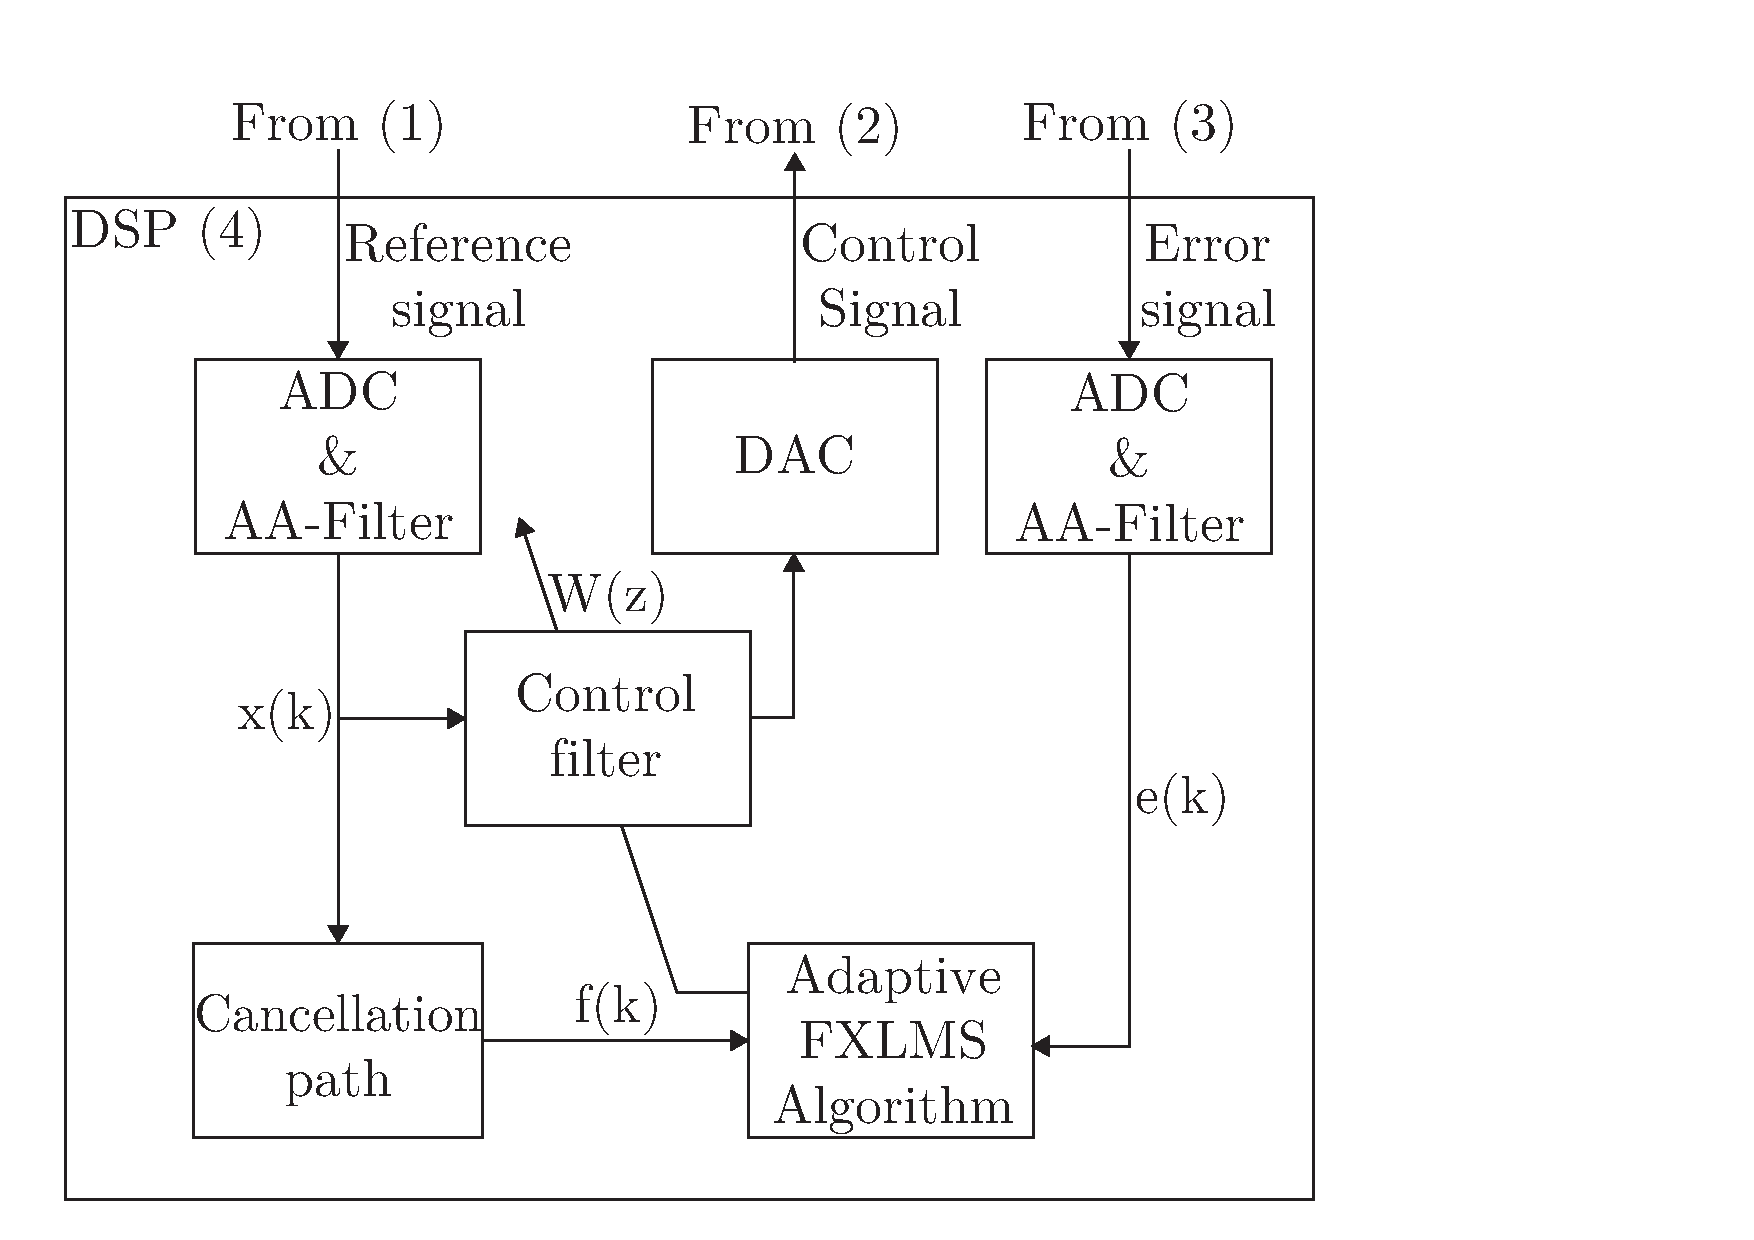
\includegraphics[width=1\columnwidth]{figures/ArticleIllustrations/ANCFeedForward}
		\tikzsetnextfilename{ANCFeedForward}
		\resizebox{0.95\columnwidth}{!}{
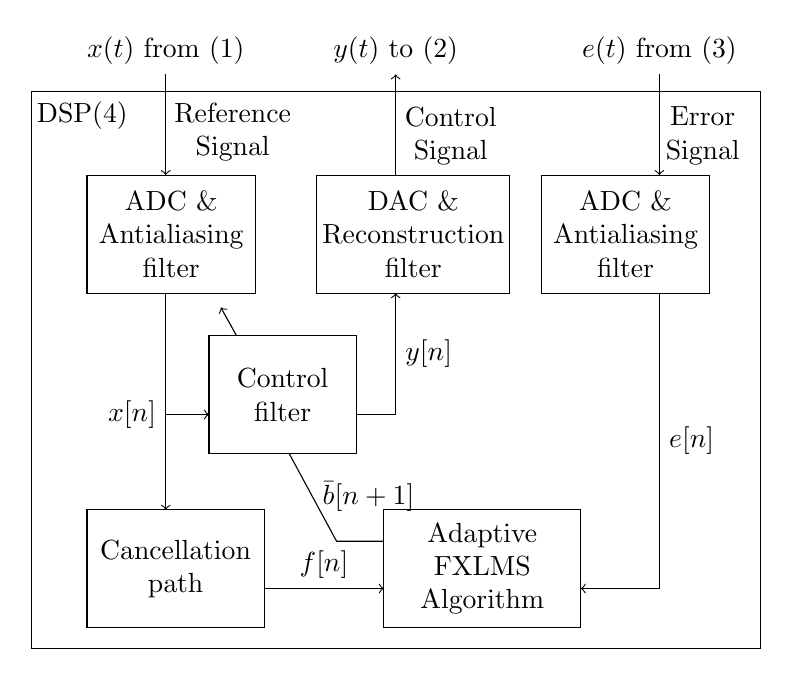
\begin{tikzpicture}
\draw  (-3,4.93) rectangle node[text width=2cm,align=center] {ADC \& Antialiasing filter} (-0.86,3.43);
\draw  (-3,0.68) rectangle node[text width=2.5cm,align=center] {Cancellation \\ path}(-0.75,-0.82);
\draw  (0.77,0.68) rectangle node[text width=2.5cm,align=center] {Adaptive FXLMS Algorithm} (3.27,-0.82);

\draw  (-1.45,2.89) rectangle node[text width=1.5cm,align=center,fill=white] {Control filter} (0.42,1.39);
\draw  (-0.08,4.93) rectangle node[text width=2.5cm,align=center] {DAC \& \\ Reconstruction filter}(2.37,3.43);
\draw  (2.77,4.93) rectangle node[text width=2cm,align=center] {ADC \& Antialiasing filter}(4.91,3.43);

\draw  (-3.71,5.99) rectangle (5.55,-1.08);
\node at (-3.06,5.69) {DSP(4)};
\node [text width=2cm,align=center] at (-1.15,5.48) {Reference Signal};

\draw[->] (-0.75,-0.32) -- node[above]{$f[n]$} (0.77,-0.32);

\draw[->] (4.27,3.43) -- node[right]{$e[n]$} (4.27,-0.32)  -- (3.27,-0.32);

\draw [->](4.27,6.21) node[above]{$e(t)$ from (3)} -- (4.27,4.93) ;
\draw [->](0.92,4.93)  --  (0.92,6.21) node[above]{$y(t)$ to (2)};
\draw [->](-2,3.43) -- (-2,0.68);

\draw [->](-2,1.89) node[left]{$x[n]$} -- (-1.45,1.89);

\draw[->] (0.42,1.89) -- (0.92,1.89) --node[right]{$y[n]$} (0.92,3.43);
\draw [->](-2,6.21) node[above]{$x(t)$ from (1)} -- (-2,4.93);
\node [text width=2cm,align=center] at (1.62,5.43) {Control Signal};
\node [text width=1.5cm,align=center] at (4.82,5.43) {Error Signal};

\draw (0.77,0.28) -- (0.17,0.28) --node[above=0.25,right]{$\bar{b}[n+1]$} (-0.43,1.39);
\draw [->](-1.1,2.89) -- (-1.3,3.25);
\end{tikzpicture}}
	\caption{Block diagram of adaptive feedforward ANC system.}
	\label{fig:ANCFeedforward}
\end{figure}

The signals from (1) and (3) from \autoref{fig:ANCFeedforward} are converted to the digital domain using an ADC and anti-aliasing (AA) filters before processing. When processed, the output $y[n]$ is reconstructed using a DAC. \\\\

%\begin{figure}[H]
%	\centering
%	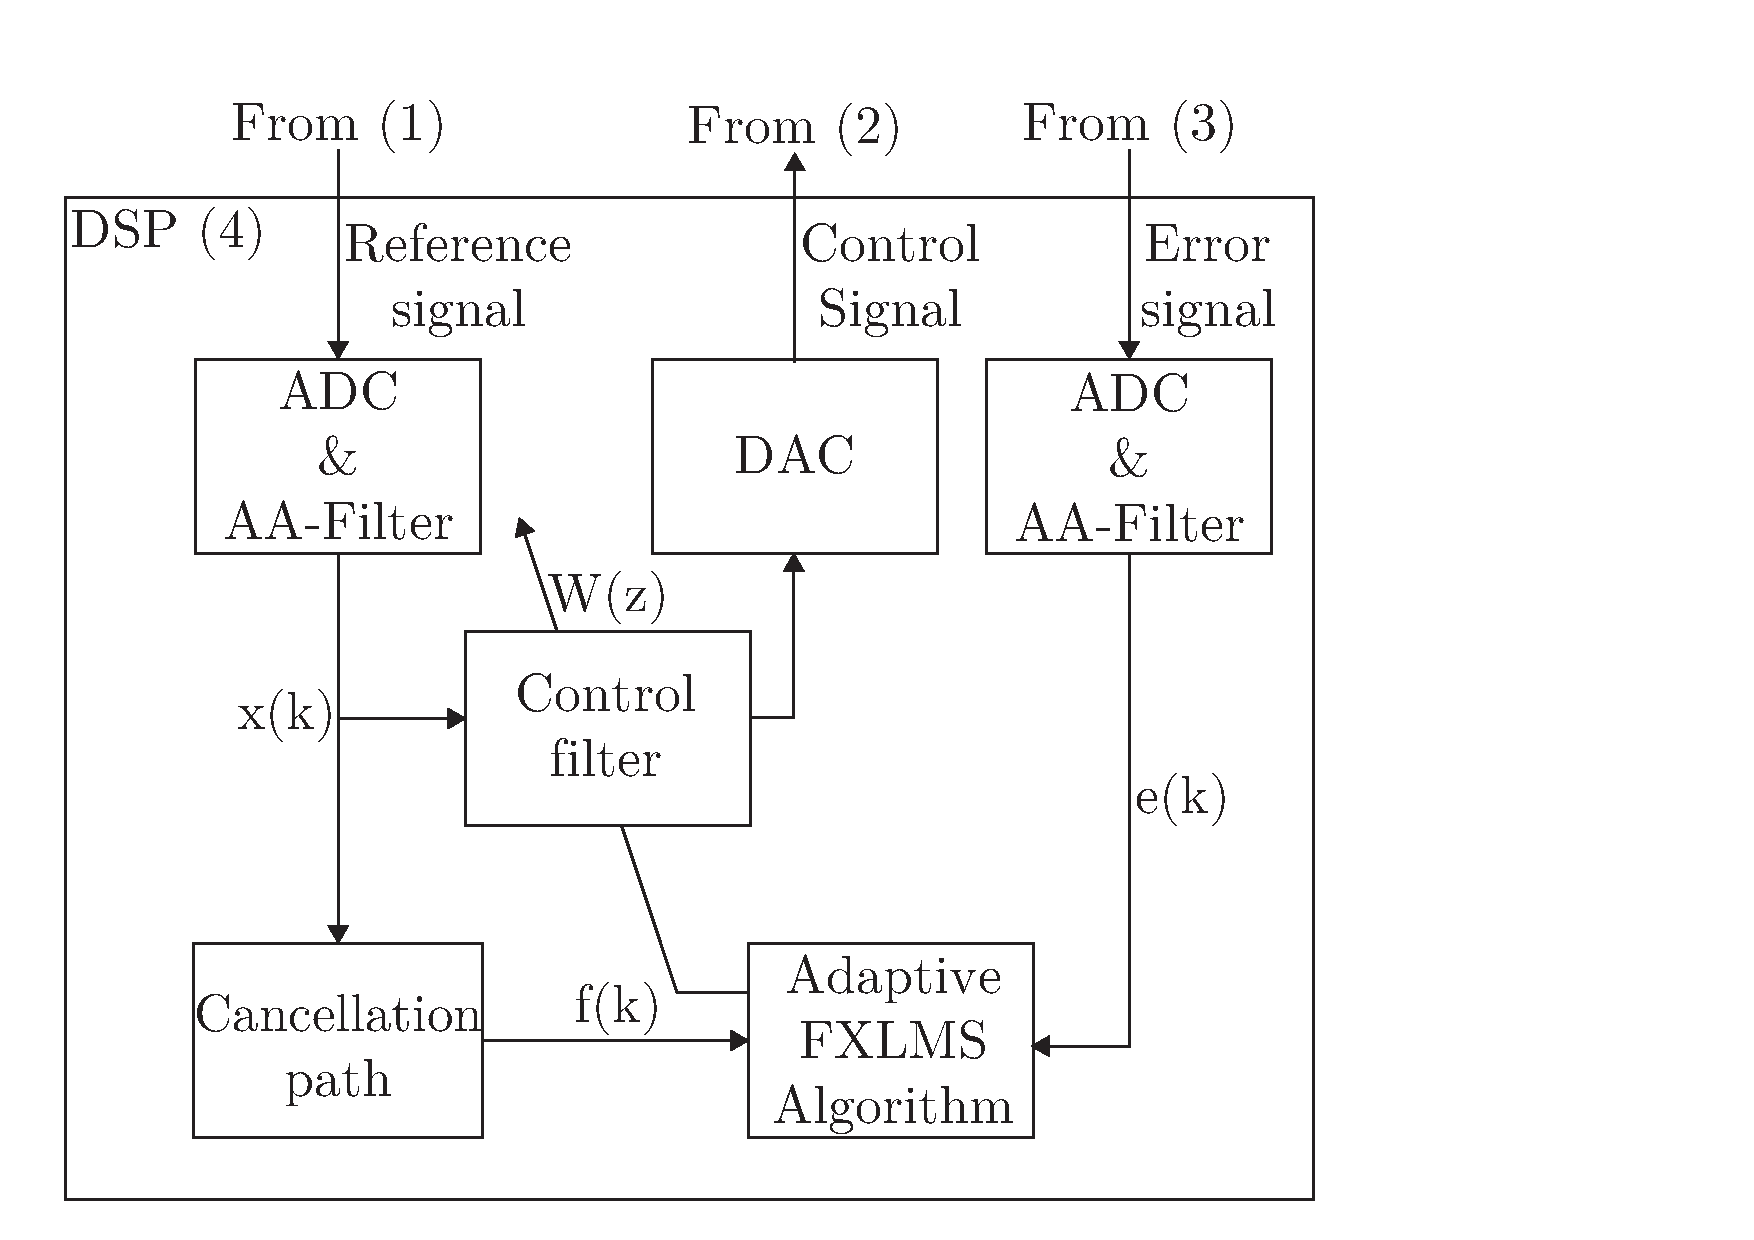
\includegraphics[width=1\columnwidth]{figures/ArticleIllustrations/ANCFeedForward}
%	\caption{Adaptive feedforward ANC system}
%	\label{fig:ANCFeedforward}
%\end{figure}

The Control Filter, shown in \autoref{eq:Output}, is initialized with the inverse of the measured impulse response of the represented transfer function. An order of 960 taps is chosen to represent frequencies down to 50 Hz with a $f_s$ of 48 $k$Hz.
%NO fucks given!
\begin{equation}\label{eq:Output}
y[n]=\sum_{j=0}^{L-1}b_j[n]x[n-j]
\end{equation}
Where: $b_j[n]$ are the weight coefficients written as  $b[n]=[b_0[n],b_1[n], \dotsc, b_{L-1}[n]]^T$. FXLMS updates the control filter coefficients using the FXLMS method shown in \autoref{eq:FXLMS}.
\begin{equation}\label{eq:FXLMS}
b_j[n+1] = b_j[n] - 2\mu e[n]f[n-j]
\end{equation}
Where: $\mu$ is the convergence factor, $e[n]$ is the error and $f[n]$ is the reference signal convolved with the Cancellation Path (CP) shown in \autoref{eq:CP}.
\begin{equation}\label{eq:CP}
f[n]=\sum_{j=0}^{L-1}c_jx[n-j]
\end{equation}
Where: $c_j$ is the coefficient of a measured transfer-function from the headphone loudspeaker to the error microphone in the ear of a Head and Torso Simulator (HATS). In the literature \cite{Hansen} the CP is adaptively adjusted, but it is assumed constant because the position of the headphone does not change while measured on a HATS. This assumption is made because it is irrelevant for verifying if LP is a plausible solution. 


%When implementing the system, delays exist due to the anti-aliasing and reconstruction filters. The delays of the system exceeds the propagation time of sound from the reference microphone to the headphone loudspeaker resulting in poor performance. Therefore an LP-algorithm is proposed to predict future samples in order to decrease the effect of the time delays.



\subsection{Characteristics of Speech}
Speech is characterized quasiperiodic signal which can be split into two main classes; voiced and unvoiced. Voiced sounds are characterized by a strong periodicity, with the fundamental frequency referred to as the pitch frequency (50 Hz-500 Hz). Unvoiced sounds are characterized as stochastic. Speech is a non stationary signal and can only be assumed Wide Sense Stationary (WSS) for periods of 20 $m$s-30 $m$s \cite{Speech}. 

\subsection{Linear Prediction of Speech}
The outlines of the prediction system is shown in figure \ref{fig:LinearPredictionOverview}. The system predicts $\hat{x}[n+P]$ by adapting linear prediction coefficients (LPCs) $\hat{\bar{a}}$, in a Wiener filter, determined using a framebased Auto Correlation Function (ACF) $\hat{r}_x[l]$ \cite{LinearPrediction}.   

\begin{figure}[H]
	\centering
	\tikzsetnextfilename{WienerHopf}
	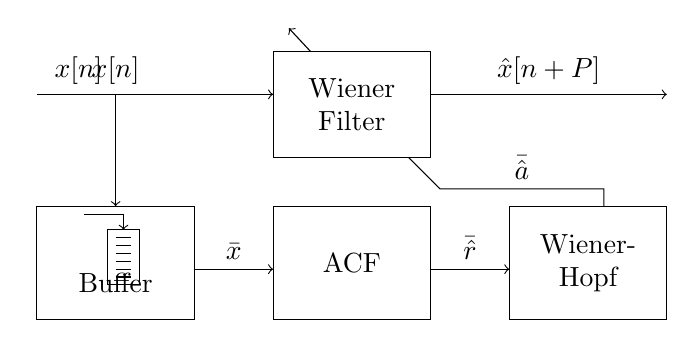
\begin{tikzpicture}

%% Boxes
\draw  (-3,3) rectangle node[text width=2cm,align=center] {Wiener Filter}(-1,4.34);
\draw  (-1,2.38) rectangle node[text width=2cm,align=center] {ACF}(-3,0.94);
\draw  (-4,2.38) rectangle node[text width=2cm,align=center,below=.25] {Buffer}(-6,0.94);
\draw  (0,2.38) rectangle node[text width=1.5cm,align=center] {Wiener- Hopf}(2,0.94);



%%Buffer
\draw (-4.7,1.38) node (v1) {} -- (-5.1,1.38) -- (-5.1,2.08) -- (-4.7,2.08) -- (-4.7,1.38);
\draw (-5,1.98) -- (-4.8,1.98);
\draw (-5,1.88) -- (-4.8,1.88);
\draw (-5,1.78) -- (-4.8,1.78);
\draw (-5,1.68) -- (-4.8,1.68);
\draw (-5,1.58) -- (-4.8,1.58);
\draw (-5,1.48) -- (-4.8,1.48);
\draw [->](-5.4,2.28) -- (-4.9,2.28) -- (-4.9,2.08);


%% Lines
\draw [->](-4,1.58) -- node[above]{$\bar{x}$} (-3,1.58);
\draw [->](-1,1.58) -- node[above]{$\bar{\hat{r}}$}(0,1.58);
\draw (1.2,2.38) -- (1.2,2.6) -- node[above]{$\bar{\hat{a}}$} (-0.88,2.6) -- (-1.28,3);


\draw [->](-2.52,4.34) -- (-2.8,4.64);
\draw [->](-6,3.8) node[right=15,above]{$x[n]$} -- (-3,3.8);
\draw [->](-5,3.8) node[above]{$x[n]$} -- (-5,2.38);
\draw [->](-1,3.8) --  node[above]{$\hat{x}[n+P]$}(2,3.8);
\end{tikzpicture}
	%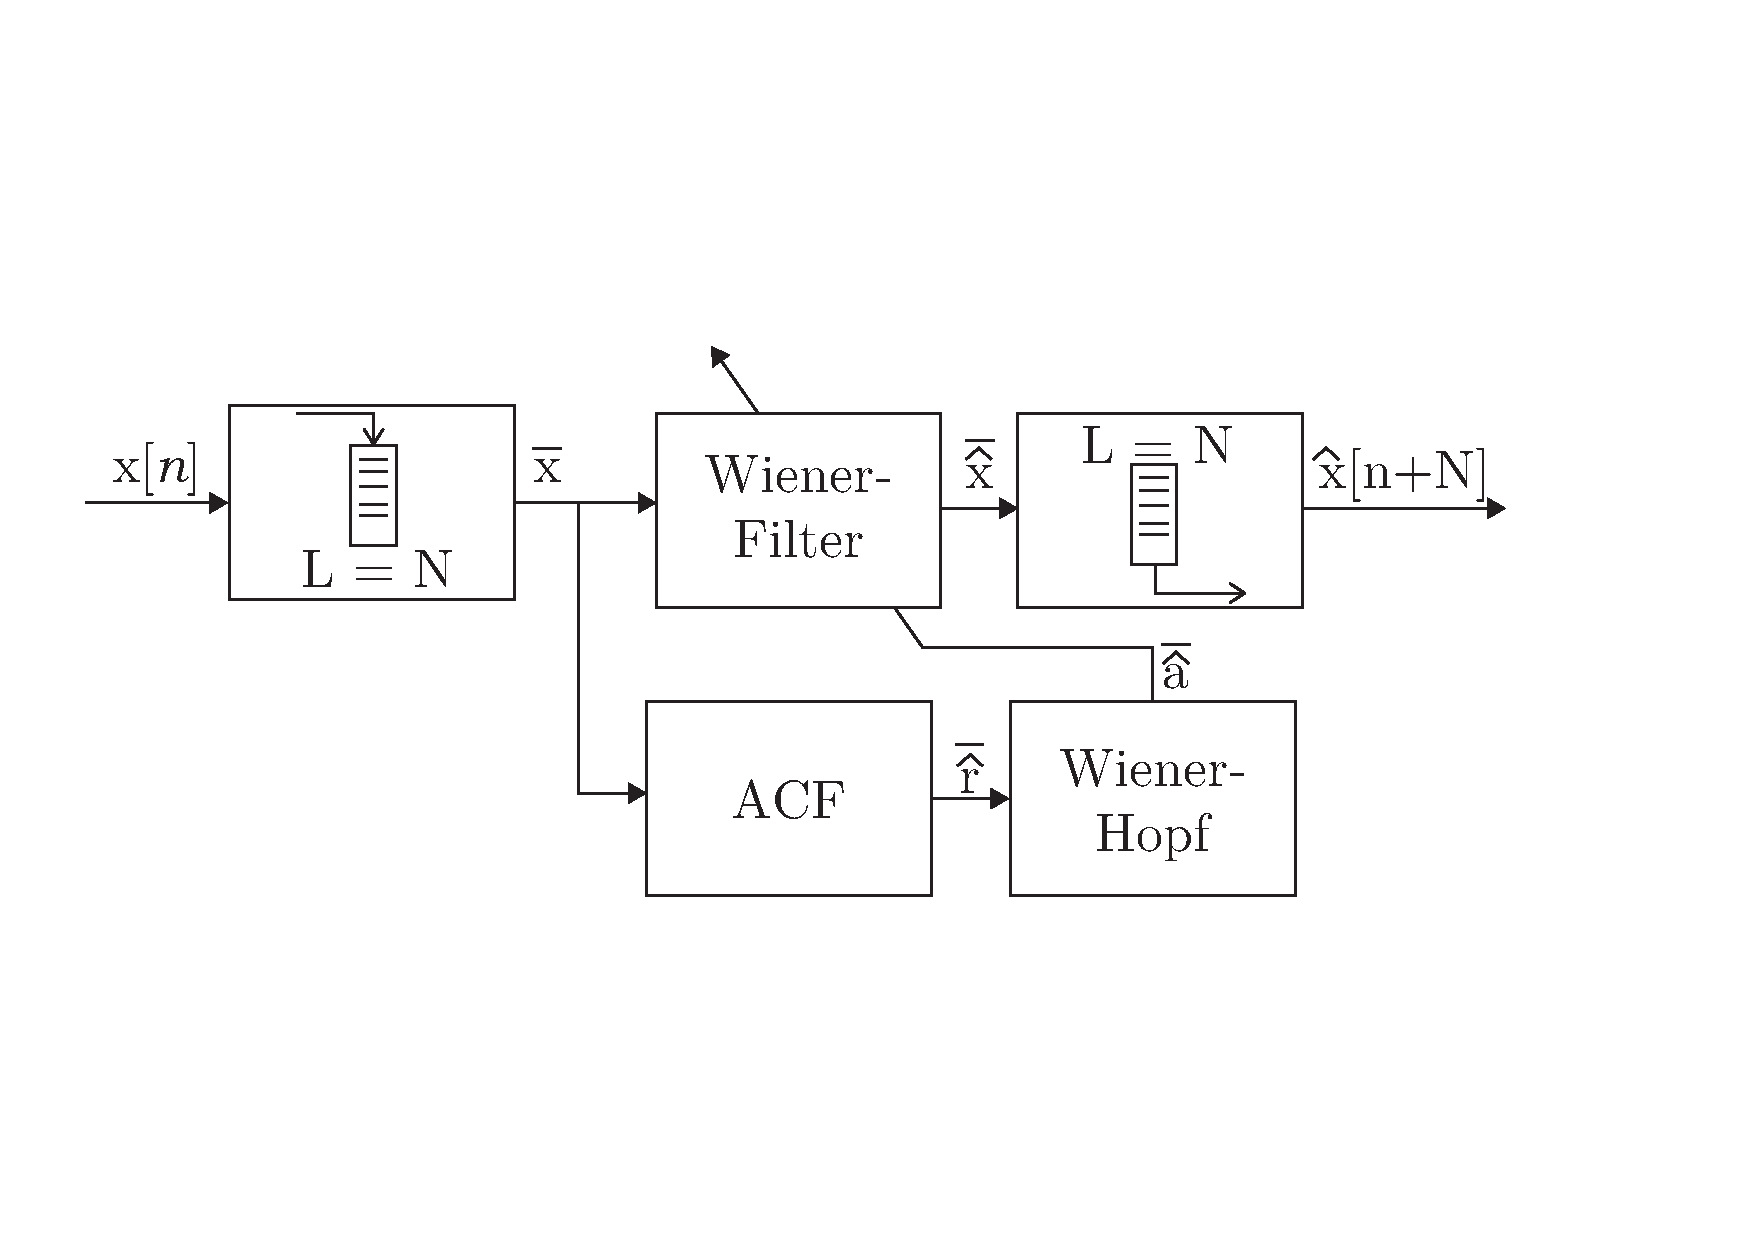
\includegraphics[width=\columnwidth]{figures/ArticleIllustrations/WienerHopf}
	\caption{Block diagram of linear prediction system.}
	\label{fig:LinearPredictionOverview}
\end{figure}


The ACF is estimated by nonrecursive estimation, shown in \autoref{eq:nonrecursive}, with framelength N. The nonrecursive estimation relies on a well defined window in order to increase the periodicity of the ACF. This is done by weighting the center of the frame highest, assuming highest periodicity in the center of a frame. Therefore a Hamming window, w is applied being one of the most widely used in speech encoding \cite{LinearPrediction}. Furthermore overlapping, $O$ can be used to increase the update rate of the ACF without having a small framelength.  
\begin{equation}\label{eq:nonrecursive}
%%r_x[l,m] = \sum^{m}_{n=m-N+1+\left| l\right|} x_l[n]w_l[m-n]
\hat{r}_x[l] = \sum^{N}_{n=\left| l\right|} x_l[n]w_l[N-n]
\end{equation}
%\begin{multline}\label{eq:nonrecursive}
%R[l,m] = \sum^{m}_{n=m-N+1+\left| l\right|} \\ x[n]w[m-n] x[n-\left| l\right|]w[m-n+\left| l\right|]
%\end{multline}
%\begin{equation}
%R[l,m]=\sum^{m}_{n=m-N+1+\left| l\right|}x[n]w[m-n] x[n-\left| l\right|]w[m-n+\left| l\right|]
%\end{equation}
Where: l is the lag, $x_l[n]=x[n]x[n-l]$ and $w_l[n]=w[n]w[n+l]$. The LPCs are determined using \autoref{eq:normal}, known as the Wiener-Hopf equation.
\begin{equation}\label{eq:normal}
\hat{R}  \bar{a} = -\bar{\hat{r}}_x
\end{equation}
Where: $\hat{R}$ is the covariance matrix $\hat{C}_{xx}$, $\bar{\hat{a}}$ is the LPCs $\bar{\hat{a}} = [\hat{a}_0 , \hat{a}_1, \dotsc, \hat{a}_{N-1}]^T$ and $\bar{\hat{r}}_x$ is the ACF, $\bar{\hat{r}}_x = [\hat{r}_x[1] , \hat{r}_x[2], \dotsc, \hat{r}_x[N]]^T$. \autoref{eq:normal} can be rewritten as shown in \autoref{eq:normal2} yielding the LPCs directly.  
 \begin{equation}\label{eq:normal2}
\bar{\hat{a}} = \hat{-R^{-1}} \bar{\hat{r}}_x
\end{equation}
Calculating $\hat{R}^{-1}$ is computationally heavy on a DSP. Therefore to estimate the LPCs the Levinson-Durbin method is used \cite{LinearPrediction}. Prediction using Wiener filtering, shown in equation \ref{eq:Predictor}, can then be applied to the current frame for prediction of the next frame. To decrease the computational cost only LPCs with an impactfull magnitude should be used. These are the first 50-400 LPCs and the LPCs located at the respective pitch frequency of the speech \cite{Speech}.      

\begin{equation}\label{eq:Predictor}
\hat{x}[n+p] =- \sum^{M-1}_{i=1}\hat{a}_i[n]x[(n+p)-i]
\end{equation}

Using equation \ref{eq:Predictor} in cascade where $\hat{x}[n+2]$ is estimated using $\hat{x}[n+1]$ and $x[n]$ up until $\hat{x}[n+P]$. 


\subsection{Prediction Gain}
For the purpose of testing the LP's prediction gain (PG) shown in \autoref{eq:PG} will be used. 
\begin{equation}\label{eq:PG}
PG = 10 log_{10}\bigg(\frac{\sigma^2_x}{\sigma^2_\varepsilon}\bigg) = 10 log_{10}\bigg(\frac{E\{x^2[n]\}}{E\{\varepsilon^2[n]\}}\bigg)
\end{equation}
Where: PG is the ratio between the variance of the input signal $x[n]$ and the variance of the prediction error, $\varepsilon$ measured in dB. The higher the PG the better the prediction is.



\subsection{Feedforward LP FXLMS}
The adaptive ANC system combined with the predictor is shown on \autoref{fig:LPFXLMS}. Here the predictor will be inserted before the ANC system. The predictor need to compensate for both the ADC delay and the DAC delay, which are assumed to have the same delay ($i=\frac{P}{2}$).   

\begin{figure}[H]
	\centering
	\tikzsetnextfilename{CombinedSystem2}
	\resizebox{1\columnwidth}{!}{
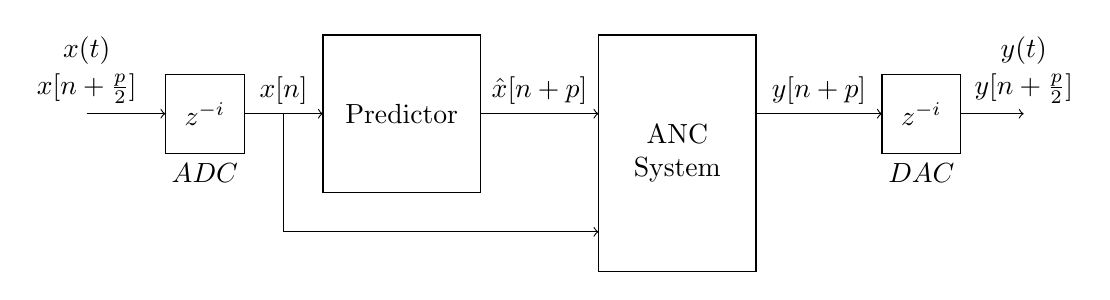
\begin{tikzpicture}
\draw  (-4,1.5) rectangle node {$z^{-i}$} (-5,0.5);
\draw (-4.5,0) node[above]{$ADC$} ;

\draw  (-3,2) rectangle  node[align=center] {Predictor} (-1,0) ;

\draw  (0.5,2) rectangle node[text width=1.5cm,align=center] {ANC System}(2.5,-1);
\draw  (4.1,1.5) rectangle node {$z^{-i}$}(5.1,0.5);
\draw (4.6,0) node[above]{$DAC$} ;

\draw [->](-4,1)  -- (-3,1);


\draw [->](-1,1)  -- node[above]{$\hat{x}[n+p]$}  (0.5,1);
\draw [->](2.5,1) -- node[above]{$y[n+p]$} (4.1,1);

\draw [->](-6,1) node[above]{$x[n+\frac{p}{2}]$} -- (-5,1);
\draw (-6,1.5) node[above]{$x(t)$} ;
\draw [->](5.1,1)-- (5.9,1) node[above]{$y[n+\frac{p}{2}]$} ;
\draw [->](-3.5,1) node[above]{$x[n]$} -- (-3.5,-0.5) -- (0.5,-0.5);
\draw (5.9,1.5) node[above]{$y(t)$} ;
\end{tikzpicture}}
	\caption{Block diagram of combined system of LP and feedforward FXLMS.}
	\label{fig:LPFXLMS}
\end{figure}

The adaptive ANC inputs the predicted input $\hat{x}[n+P]$ and the measured input $x[n]$, into the control filter and the CP. This will expand \autoref{eq:Output} and \autoref{eq:CP} into \autoref{eq:ControlExpanded} and \autoref{eq:CPExpanded} respectively.   

\begin{equation}\label{eq:ControlExpanded}
y[n+P]=\sum^{P-1}_{j=0}b_j[n]\hat{x}[(n+P)-j]+\sum^{L-1}_{j=P}b_j[n]x[(n+P)-j]
\end{equation}

\begin{equation}\label{eq:CPExpanded}
f[n+P]=\sum^{P-1}_{j=0}c_j\hat{x}[(n+P)-j]+\sum^{L-1}_{j=P}c_jx[(n+P)-j]
\end{equation}

The reasoning behind using both $\hat{x}[n+P]$ and $x[n]$ is that it will give a more precise result, than if only $\hat{x}[n+P]$ was used in the ANC system. This is because less predicted samples will be input into the ANC system which should result in a more precise $y[n+P]$. The input $e[n]$ is not predicted because the proposed solution of delaying $f[n+P]$ $i$ times, is easier. This results in $f[n+\frac{P}{2}]$ which coincides with $e[n+\frac{P}{2}]$ as shown on \autoref{fig:LPFXLMS}. Delaying instead of predicting will yield a slower reaction time however it is much less computationally heavy for a DSP.       

